\chapter{Проектирани печатни платки}
\label{boards_chapter}
%\section{Функции и параметри}  %явява се повторение
%адаптер
%индикация
%захранване
\section{Принципна електрическа схема}
\subsection{PATA адаптер и тестов адаптер}
Тестовият адаптер свързва оригиналният кабел на РОБКО 01 с микроконтролерната платка. Отделните проводници от кабела са запоени адаптерната платка и са свързани към стандартен двуредов конектор. Сигналите \textoverline{DINE} и \textoverline{BS} не са изведени, а сигналите A4-A7 се свързват към външни установяващи съпротивления върху прототипна платка. Този адаптер е използван само за тестване на разработката преди да бъдат произведени другите две платки.

Серията РОБКО разполага със собствен специфичен конектор. Броят пинове на този конектор и на стандартния PATA конектор съвпадат. Това позволява РОБКО 01 да се свързва към управляващо устройство през стандартен PATA лентов кабел с подходящ адаптер. Това е функцията на втората платка от настоящата система. Всеки проводник от РОБКО конектора е свързан със съответен проводник от PATA конектора. Изключение прави средният ред на РОБКО конектора. Тези проводници са свързани заедно и към същия брой пинове в PATA конектора. В различните портове на РОБКО 01 те са свързани или към земя или към захранване, но винаги всички заедно.\\
\indent{}
РОБКО/PATA адаптерът е двустранна платка. От едната страна е PATA конекторът, а от другата РОБКО конекторът или три стандартни едноредови конектори. Поставя се директно в порт B на РОБКО 01. Може да се използва и за порт A на РОБКО 01.
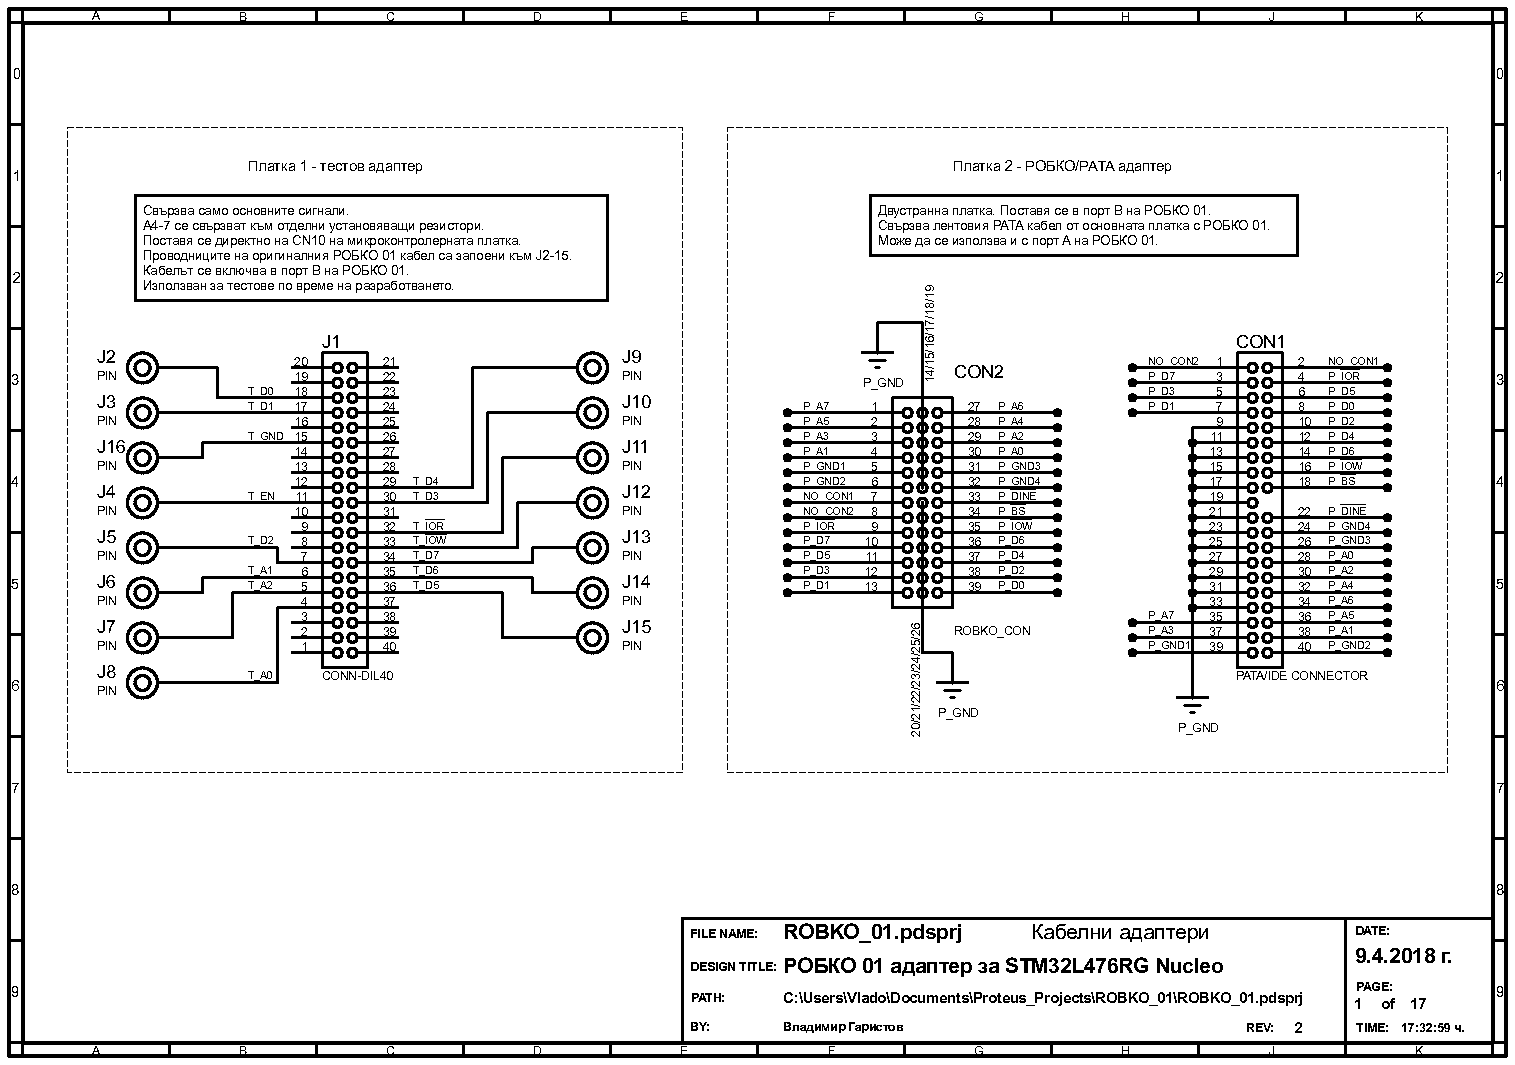
\includepdf[pages={1},angle=90]{documents/schematic_bw.pdf}
\subsection{Захранващ блок}
Захранващият блок е част от основната платка. SW3 е главният прекъсвач. През него протича захранващият ток за РОБКО 01 и за микроконтролерната платка. Схемата черпи енергия от 12-волтов източник, свързан към конектор J21. Конектор J22 подава напрежение на РОБКО 01, а конектор J23 на оптичният сензорен хващач. Микроконтролерната платка се захранва през конектор J17, показан на схемна страница "Конектори и индикация". През същия конектор основната платка получава 3,3V захранващо напрежение от линеен регулатор на микроконтролерната платка. С 3,3V се захранват джойстиците.\\
\indent{}
Захранването включва три защити - против късо съединение, против пренапрежение и против грешен поляритет на напрежението. Защитата от късо съединение се реализира с два 5-амперови бушона. Първият от тях обхваща РОБКО 01 и микроконтролерната платка, а другият само робота. Бушоните са бавнодействащи с цел да се избегне изгарянето им при кратки токови импулси, породени от индуктивния характер на моторите. Защитата против пренапрежение се осъществява чрез двупосочен трансил с номинално пробивно напрежение 13,3 V. Защитата от грешен поляритет на захранващото напрежение се реализира от P-канален MOSFET Q1, ценеров диод D7 и резистор R17. При правилен поляритет на напрежението протича ток през паразитния диод на Q1. D7 и R17 образуват делител на напрежение. Напрежението гейт-сорс на Q1 става равно на пробивното напрежение на D7 и транзисторът се отпушва. Ако на схемата се подаде отрицателно захранващо напрежение, диодът на Q1 се явява свързан в обратна посока и транзисторът остава запушен.\\
\indent{}
Микроконтролерната платка и оптичният сензорен хващач се захранват от U1 - линеен регулатор на напрежение 7805 с максимален ток 1,5A. Двете захранващи напрежения +12V и +5V се стабилизират от по един 100$\mu$F кондензатор. Монтажните отвори са заземени. През металните болтове и отстъпи те се свързват електрически с металното шаси на захранващия източник, а през него и със заземяващия проводник на сградната електроинсталация.
\includepdf[pages={3},angle=90]{documents/schematic_bw.pdf}
\subsection{Връзка между STM32L476RG и РОБКО 01}

Основната платка играе ролята на централен възел, свързващ другите компоненти на системата. Конектори CN7 и CN10 на микроконтролерната платка се свързват съответно с конектори J17 и J20 от основната. Конектори J17 и J20 се намират на страна спойки с цел микроконтролерната платка да се поставя под основната. Двете платки се прикрепят една към друга и към корпуса на захранващия източник с помощта на метални отстъпи и болтове. В конектор CON3 на основната платка се поставя единия край на лентовия PATA кабел към РОБКО 01. Резисторите R1-R4 установявят адресните сигнали A4-A7. Конектори J18 и J19 се свързват с USB-UART конверторната платка, която се свързва с компютъра изпълняващ сървърния софтуер.
\subsection{Индикация}
Светодиодите D1-D6 предоставят визуална индикация на състоянията на стъпковите мотори. Диод D1 съответства на мотор 0, D2 на мотор 1 и т.н. Номерата на моторите са обозначени на ситопечата от страна компоненти на платката и в таблица \ref{tab:addr_space}. Светодиодите са по два в корпус - зелен и червен. Зеленият цвят означава движение напред, а червеният - движение назад. При неподвижен мотор съответните светодиоди не светят.
\subsection{Ръчно управление}
\label{manual_cntrl_section}
Джойстиците за ръчно управление се описват подробно в точка \ref{joysticks}. Кабелите им се свързват към конектори RJ1 и RJ2. За определяне на ориентацията на джойстиците се използва вградения в микроконтролера аналогово-цифров преобразувател. Различните режими на управление се конфигурират от прекъсвачите SW1.\\
\indent{}
Първият прекъсвач (обозначен с единица върху корпуса на компонента; между пинове 4 и 5 на схемата) конфигурира скоростта на въртене на моторите. Когато е отворен е избрана бавна скорост, а когато е затворен - бърза. Чрез вторият прекъсвач се избира дали стъпковите мотори да се задвижват в режим на пълна стъпка (отворен) или на полустъпка (затворен). Третият прекъсвач се взима под внимание само ако четвъртият е отворен. Чрез него се избира режима на управление, като отворен съответства на отдалечено управление, а затворен на ръчно. Последният прекъсвач включва възможността на микроконтролера да засича дали двата джойстика са свързани към платката и ако са, автоматично да премине в ръчен режим.
При отворен прекъсвач тази функционалност е изключена.
%добави RPM
Бутонът SW2 рестартира микроконтролера.
\includepdf[pages={2},angle=90]{documents/schematic_bw.pdf}
\section{Графични оригинали на печатните платки}
Всички графични оригинали са в отношение 1:1 спрямо физически реализираните печатни платки.\\
Тестовият адаптер е ръчно изработен на базата на фабрично пробита и метализирана прототипна платка. Другите две печатни платки са произведени машинно.
\FloatBarrier
\subsection{Тестов адаптер}
\begin{figure}[!htbp]
    \begin{minipage}{0.49\linewidth}
        \centering
        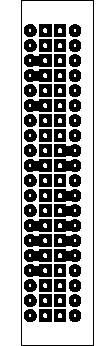
\includegraphics[page=1]{documents/dev_board.pdf}
        \caption{Страна спойки}
        \label{fig:dev_top}
    \end{minipage}
    \hfill
    \begin{minipage}{0.49\linewidth}
        \centering
        \includegraphics[page=2]{documents/dev_board.pdf}
        \caption{Страна компоненти}
        \label{fig:dev_bot}
    \end{minipage}
\end{figure}
\begin{figure}[!htbp]
    \begin{minipage}{0.49\linewidth}
        \centering
        \includegraphics[page=3]{documents/dev_board.pdf}
        \caption{Ситопечат,\\страна спойки}
        \label{fig:dev_top_silk}
    \end{minipage}
    \hfill
    \begin{minipage}{0.49\linewidth}
        \centering
        \includegraphics[page=4]{documents/dev_board.pdf}
        \caption{Ситопечат,\\страна компоненти}
        \label{fig:dev_bot_silk}
    \end{minipage}
\end{figure}
\begin{figure}[!htb]
    \begin{minipage}{0.49\linewidth}
        \centering
        \includegraphics[page=5]{documents/dev_board.pdf}
        \caption{Изолационен лак,\\страна спойки}
        \label{fig:dev_top_res}
    \end{minipage}
    \hfill
    \begin{minipage}{0.49\linewidth}
        \centering
        \includegraphics[page=6]{documents/dev_board.pdf}
        \caption{Изолационен лак,\\страна компоненти}
        \label{fig:dev_bot_res}
    \end{minipage}
\end{figure}
\begin{figure}[!htb]
    \begin{minipage}{0.49\linewidth}
        \centering
        \includegraphics[page=7]{documents/dev_board.pdf}
        \caption{Очертание\\на печатната платка}
        \label{fig:dev_cont}
    \end{minipage}
    \hfill
    \begin{minipage}{0.49\linewidth}
        \centering
        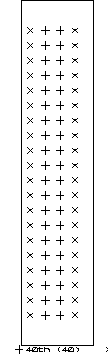
\includegraphics[page=1]{documents/dev_board_drill.pdf}
        \caption{Отвори}
        \label{fig:dev_drill}
    \end{minipage}
\end{figure}
\FloatBarrier
\subsection{PATA адаптер}
\begin{figure}[!htb]
    \begin{minipage}{0.49\linewidth}
        \centering
        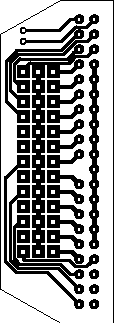
\includegraphics[page=1]{documents/pata_board.pdf}
        \caption{Страна компоненти}
        \label{fig:pata_top}
    \end{minipage}
    \hfill
    \begin{minipage}{0.49\linewidth}
        \centering
        \includegraphics[page=2]{documents/pata_board.pdf}
        \caption{Страна спойки}
        \label{fig:pata_bot}
    \end{minipage}
\end{figure}
\begin{figure}[!htbp]
    \begin{minipage}{0.49\linewidth}
        \centering
        \includegraphics[page=3]{documents/pata_board.pdf}
        \caption{Ситопечат,\\страна компоненти}
        \label{fig:pata_top_silk}
    \end{minipage}
    \hfill
    \begin{minipage}{0.49\linewidth}
        \centering
        \includegraphics[page=4]{documents/pata_board.pdf}
        \caption{Ситопечат,\\страна спойки}
        \label{fig:pata_bot_silk}
    \end{minipage}
\end{figure}
\begin{figure}[!htbp]
    \begin{minipage}{0.49\linewidth}
        \centering
        \includegraphics[page=5]{documents/pata_board.pdf}
        \caption{Изолационен лак,\\страна компоненти}
        \label{fig:pata_top_res}
    \end{minipage}
    \hfill
    \begin{minipage}{0.49\linewidth}
        \centering
        \includegraphics[page=6]{documents/pata_board.pdf}
        \caption{Изолационен лак,\\страна спойки}
        \label{fig:pata_bot_res}
    \end{minipage}
\end{figure}
\begin{figure}[!htbp]
    \begin{minipage}{0.49\linewidth}
        \centering
        \includegraphics[page=7]{documents/pata_board.pdf}
        \caption{Очертание на\\печатната платка}
        \label{fig:pata_cont}
    \end{minipage}
    \hfill
    \begin{minipage}{0.49\linewidth}
        \centering
        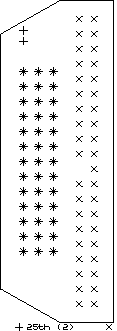
\includegraphics[page=1]{documents/pata_board_drill.pdf}
        \caption{Отвори}
        \label{fig:pata_drill}
    \end{minipage}
\end{figure}
\FloatBarrier
\subsection{Основна платка}
\begin{figure}[!htbp]
    \centering
    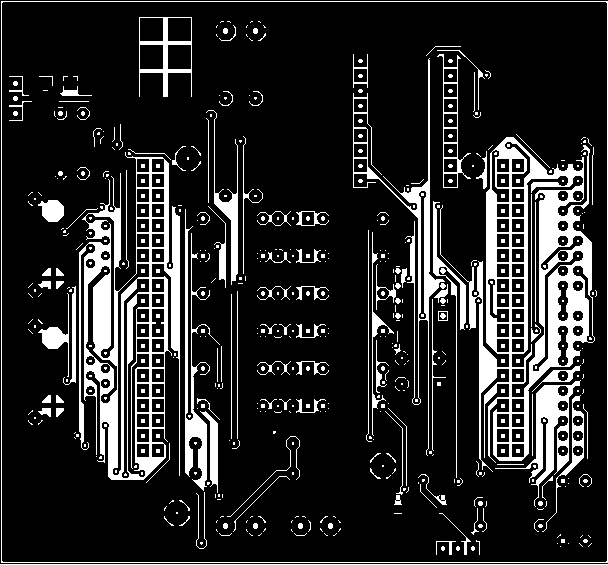
\includegraphics[page=1]{documents/main_board.pdf}
    \caption{Страна компоненти}
    \label{fig:main_top}
\end{figure}
\begin{figure}[!htbp]
    \centering
    \includegraphics[page=2]{documents/main_board.pdf}
    \caption{Страна спойки}
    \label{fig:main_bot}
\end{figure}
\begin{figure}[!htbp]
    \centering
    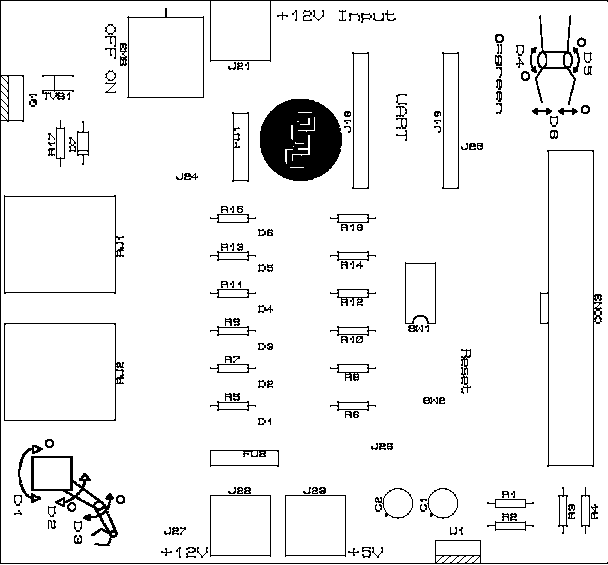
\includegraphics[page=1]{documents/top_silk.pdf}
    \caption{Ситопечат, страна компоненти}
    \label{fig:main_top_silk}
\end{figure}
\begin{figure}[!htbp]
    \centering
    \includegraphics[page=4]{documents/main_board.pdf}
    \caption{Ситопечат, страна спойки}
    \label{fig:main_bot_silk}
\end{figure}
\begin{figure}[!htbp]
    \centering
    \includegraphics[page=5]{documents/main_board.pdf}
    \caption{Изолационен лак, страна компоненти}
    \label{fig:main_top_res}
\end{figure}
\begin{figure}[!htbp]
    \centering
    \includegraphics[page=6]{documents/main_board.pdf}
    \caption{Изолационен лак, страна спойки}
    \label{fig:main_bot_res}
\end{figure}
\begin{figure}[!htbp]
    \centering
    \includegraphics[page=7]{documents/main_board.pdf}
    \caption{Припой, страна компоненти}
    \label{fig:main_top_paste}
\end{figure}
\begin{figure}[!htbp]
    \centering
    \includegraphics[page=8]{documents/main_board.pdf}
    \caption{Очертание на печатната платка}
    \label{fig:main_cont}
\end{figure}
\begin{figure}[!htbp]
    \centering
    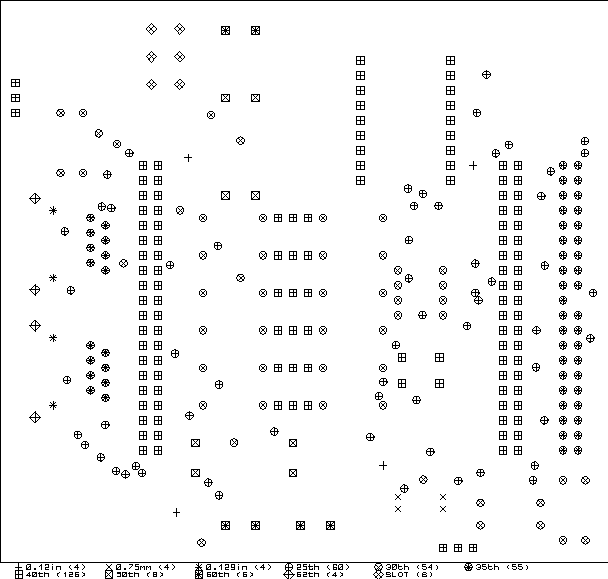
\includegraphics[page=1]{documents/main_board_drill.pdf}
    \caption{Отвори}
    \label{fig:main_drill}
\end{figure}
\FloatBarrier